%%%%%%%%%%%%%%%%%%%%%%%%%%%%%%%%%%%%%%%%%%%%%%%%%%%%%%%%%%%%%%%%%%%%%%%%%%%%%%%
% intro.tex: Introduction to the thesis
%%%%%%%%%%%%%%%%%%%%%%%%%%%%%%%%%%%%%%%%%%%%%%%%%%%%%%%%%%%%%%%%%%%%%%%%%%%%%%%%
\chapter{Introduction}
\label{chapter:intro}
%%%%%%%%%%%%%%%%%%%%%%%%%%%%%%%%%%%%%%%%%%%%%%%%%%%%%%%%%%%%%%%%%%%%%%%%%%%%%%%%

The long and winding road of a dissertation is not always neatly packaged into a template - this
can easily be seen in my own experience. While focusing much of my time on the technical aspects of
data processing software for a proposed (yet to be built) experiment, I found myself near the end
of my journey without \emph{real} data to analyze from which I can make \emph{real} conclusions
about the physical world. This motivated me to participate in another experiment -- extremely
similar to the original one -- sharing theoretical motivations, technological designs, and even
people. This experience of participating in two similar experiments has provided an abundant field
of learning opportunities (as well as roadblocks) for me and my journey as a new physicist.

Physics is a lazy science. I would go even further and state that this reductionist perspective is
a main attraction for many physicists. We\footnote{Here I use the ``royal we'' as representing my
  point of view of the culture within the field. It should in no way be construed as scientific or
  exact statements and does not represent every physicist's point of view.} want to avoid memorizing
as much as possible; therefore, motivating the idea of condensing sets of observations into
``laws'' that can be represented in an even more compact mathematical form. We make up these
``laws'' and the vocabulary surrounding them not to decieve but merely to make communication about
our observations and the experiments that make these observations easier. We sometimes debate the
origins of these laws and their true philosophical meaning, but often, on a day-to-day basis, the
background of them is unimportant. The interesting work comes from \emph{testing} them, breaking
them, and remaking them. For our purposes here, this is what a ``theory'' is: a package of laws and
their mathematical forms with which we can make predictions of the observations of our experiments.%%

While I speak in the context of all physics, in reality, I am residing within a small corner.
Primarily concerned with individual particles and how they interact with one another, my field can
be described as investigating the foundations of the universe. Our experiments require giving these
particles comparatively large amounts of energy, contextualizing the name \gls{hep-full}. Giving
such small particles such large amounts of energy requires extrodinarily large and complex
apparatuses. \gls{hep} is filled with experiments many stories tall, collaborations consisting of
hundreds of institutions and thousands of people, and observations lasting years if not decades.
This grand scale is helpful to keep in mind when I speak of the experiments in this thesis -- only
a few institutions (less than 10 in each) and only dozens of collaborators. Contrary to many other
sciences and experimental methods, these experiments still last longer than a typical doctoral
student career. While I report on these experiments, I will not detail their full operation,
design, or capabilities. I will focus on the work that I was able to contribute; hopefully
providing a building block for these experiments and \gls{hep} to grow in the future, and give only
the necessary context for parts with which I am less familiar.

Before partitioning this thesis according to the two experiments in which I participated,
\cref{sec:sm} summarizes our current laws and its representative theory that best predict our set
of observations within \gls{hep}, \cref{chapter:dm} will explore the theoretical ground on which
both of the experiments rest which will also provide necessary vocabulary for discussing these two
experiments. \cref{part:ldmx} presents the work of my initial years as a graduate student
developing data processing and realistic simulation software for a proposed experiment. This part
includes a description of this proposed experiment in \cref{chapter:ldmx:experiment}, the
simulation infrastructure for it in \cref{chapter:ldmx:simulation}, and an analysis of this
simulated data showcasing this experiment's performance in its early stages
\cref{chapter:ldmx:analysis}. \cref{part:hps} describes the work of my last years showing the
difficulties of working with data taken in the real world (with all the complexities that implies).
Similar to \cref{part:ldmx}, this part describes the experimental setup in
\cref{chapter:hps:experiment}, \todo{insert rest of chapters}. We then conclude with
\cref{chapter:conclusion} which returns back to this high-level-view from which we can discuss what
we have learned about physics via these two experiments.

\section{Standard Model of Particle Physics}
\label{sec:sm}

What makes up all the stuff around us? This question has been posed, debated, discussed, and
studied since the ancient times. Our best current understanding is that stuff is made of particles
that interact with one another. While ``particle'' is difficult to strictly define qualitatively,
we have a model for them and their interactions which we creatively named the ``Standard Model''
(SM). \cref{fig:sm} displays the known elementary particles, some of their basic properties, and
how they interact with one another. Not all of the particles represented within this diagram are of
critical importance to this work, but some deserve further description.

\begin{figure}
  \centering
  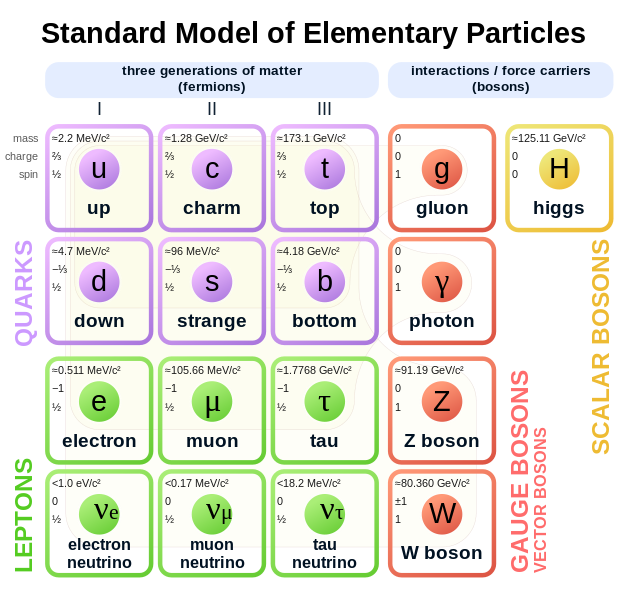
\includegraphics[width=\textwidth]{figures/intro/Standard_Model_of_Elementary_Particles.svg.png}
  \caption{
    The Standard Model of Particle Physics showing the twelve fermions and five bosons,
    their various properities (mass, charge, spin), labels (box and circle colors),
    and interactions (brown loops). Credit to Cush on wikipedia for
    providing this diagram freely accessible and usable for any purpose.
  }
  \label{fig:sm}
\end{figure}

The two lowest mass quarks -- the up and the down -- are the fundamental constituents of protons
and neutrons which make up the nuclei of atoms which make up all the day-to-day stuff we interact
with. These stay bound together within these nuclei via the strong nuclear force (mediated and
represented in the diagram by the gluon). These quarks and the top row of leptons also have an
electric charge enabling them to interact via with electromagnetic force (or equivalently exchange
photons). The electromagnetic force, represented and mediated by the photon, is the force
responsible for light and magnetism. The lowest mass charged lepton (electron) is also very
abundant -- most commonly residing in orbits around nuclei helping form atoms. Both experiments in
this thesis utilize beams of electrons that have been accelerated to high energies.

The mathematical expressions to calculate how these particles interact are complicated. As
mentioned earlier, physicists are lazy and so we have developed a method to represent the specifics
of these interactions without needing to write down any of the long mathematical formulae. These
representations are called ``Feynman diagrams'' after the 20th century physicist Richard Feynman.
Feynman diagrams allow us to represent interactions by defining a set of ``vertices'' that are
allowed by our theory and then constructing processes from these vertices that include the in- and
out- going particles that we wish to study. The further calculation of these diagrams is a defined
process that has been written into various computer programs (I say this to emphasize that these
diagrams directly represent the mathematics that can be used to calculate them).
\cref{fig:brem-feynman} shows an example Feynman diagram representing the bremsstrahlung process
where a charged lepton (\(\ell^\)) interacts with a nucleus (\(Z\)) via a photon (\(\gamma\)) and
then emits another photon before recoiling. We can see three verticies in this diagram: two
``fundamental'' vertices whree the lepton and photon lines connect and one ``effective'' vertex
where the photon connects with the nucleus. The fundamental vertices are actually strictly defined
within the Standard Model, but the effective vertex represents a helpful approximation that is
accurate at the energy scales we are studying.\footnote{ The distinction between fundamental and
  effective vertices is not a well defined one. I find it helpful here, but it is not necessarily
  made elsewhere in physics literature. }

\begin{figure}
  \centering
  \begin{tikzpicture}
    \begin{feynman}
      \vertex (in) {\(\ell^-\)};
      \vertex [right=of in] (nuc);
      \vertex [below=of nuc, blob] (nucleus) {\(Z\)};
      \vertex [right=of nuc, dot] (emit);
      \vertex [above right=of emit] (recoil) {\(\ell^-\)};
      \vertex [below right=of emit] (decay) {\(\gamma\)};
      \diagram*{
      (in) -- [fermion] (nuc) -- [fermion] (emit) -- [fermion] (recoil),
      (nucleus) -- [photon, edge label'=\(\gamma\)] (nuc),
      (emit) -- [photon] (decay),
      };
    \end{feynman}
  \end{tikzpicture}
  \caption{
    Feynman diagram for the bremsstrahlung process.
  }
  \label{fig:brem-feynman}
\end{figure}

%%%%%%%%%%%%%%%%%%%%%%%%%%%%%%%%%%%%%%%%%%%%%%%%%%%%%%%%%%%%%%%%%%%%%%%%%%%%%%%%
